\documentclass[a4paper]{article}

%% Language and font encodings
\usepackage[english]{babel}
\usepackage[utf8x]{inputenc}
\usepackage[T1]{fontenc}
\usepackage{enumitem}
\newcommand{\scala}[1]{\lstinline[basicstyle=\ttfamily\color{white},style=scala]|#1|}
%% Sets page size and margins
\usepackage[a4paper,top=3cm,bottom=2cm,left=3cm,right=3cm,marginparwidth=1.75cm]{geometry}

%% Useful packages
\usepackage{amsmath}
\usepackage{graphicx}
\usepackage{dirtytalk}
%\usepackage[colorinlistoftodos]{todonotes}
\usepackage[colorlinks=true, allcolors=blue]{hyperref}


\usepackage{beramono}
\usepackage{listings}
\usepackage{xcolor}

\definecolor{dkgreen}{rgb}{0,0.6,0}
\definecolor{gray}{rgb}{0.5,0.5,0.5}
\definecolor{mauve}{rgb}{0.58,0,0.82}
\definecolor{mygray}{rgb}{0.5,0.5,0.5}

\lstdefinestyle{scala}{
  language=scala,
  aboveskip=3mm,
  belowskip=3mm,
  showstringspaces=false,
  columns=flexible,
  basicstyle={\small\ttfamily},
  numbers=none,
  numberstyle=\tiny\color{gray},
  keywordstyle=\color{blue},
  commentstyle=\color{dkgreen},
  stringstyle=\color{mauve},
  frame=none,
  breaklines=true,
  breakatwhitespace=true,
  tabsize=3,
  numbers=left,                    % where to put the line-numbers; possible values are (none, left, right)
  numbersep=5pt,                   % how far the line-numbers are from the code
  numberstyle=\tiny\color{mygray} % the style that is used for the line-numbers
}

\title{Generic programming in Scala \\ 
\Large{Research report}\footnote{The code accompanying this research can be found at \url{https://github.com/maffh92/Concepts-of-program-design}}}
\author{Carlos Tomé Cortiñas
\and Matthew Swart
\and Renate Eilers}

\begin{document}
\maketitle

\section{Introduction}

Regular programmers may often find themselves writing the same piece of code over and over, with only the slightest variations to account for the varying datatypes their code operates on. Consider, for instance, a set of functions for  calculating the size of a datastructure such as a list or a tree. On the surface these programs will look quite different, as they are designed to work on different datatypes, but on a closer look, they are actually very similar: both recursively calculate the size of the substructures of what they are passed, and then put these results together. From the wish to end needing to repeatedly write more-or-less the same functions, the idea of \emph{datatype-generic programming} was born. Datatype-generic programming entails the writing of functions on the \emph{structure} of datatypes rather than on concrete instantiations. This would allows programmers to write a single generic function for an entire class of datatypes. The main idea here is that most datastructures can be expressed as a combination of basic structural elements, such as sums and products. Abstracting over the specifics of a datastructure allows us to see that many computations simply consists of transforming one structure into another or breaking a structure down into a single value. If such functions are then defined as operations on the structures of these aforementioned \emph{standard} types, a lot of code duplication can be foregone. 

Not every programming language lends itself for generic programming. According to \\ Gibbons\cite{Gibbons06designpatterns}, a language should allow parameterisation in three forms in order to support datatype-generic programming: by \emph{element type}, by the \emph{body} of the computation, and by \emph{shape} of the computation.

Historically, Haskell has been the popular choice for datatype-generic programming, as it supports all the aforementioned forms of parameterisation (Oliveira and Gibbons,\cite{Oliveira08scalafor}). Since Scala is gaining more and more popularity worldwide (it is ranked \#31 on the TIOBE Index\cite{tiobe}, and \#15 on the PYPL PopularitY of Programming Language Index\cite{pypl}), it would be an interesting project to see how well Scala lends itself for generic programming.

Scala\cite{odersky2004scala} is a language incorporating features from both the functional and object-oriented paradigm which runs on the Java platform. In Scala, every value is an object, and every operation is a method call. According to its creator, Martin Odersky, novel constructs such as \emph{traits} and \emph{mixin composition} allow for more advanced object composition than most other languages\cite{odersky2005scalable}. Scala facilitates the parameterisation of shape through higher-kinded types, generics take care of parameterisation by type, and parameterisation of computation can be handled using higher-order functions\cite{Oliveira08scalafor}. 

\section{Problem}
% See how well Scala lends itself for GP. One library already exists: Shapeless
% We want to see how other GP approaches port to Scala

With this research we aim to investigate Scala's potential within the domain of datatype-generic programming. For a long time, Haskell has been the go-to language for the exploration of datatype-generic programming\cite{Oliveira08scalafor}, which over time has resulted in the development of a considerable number of Haskell libraries for this purpose (e.g. GHC.Generics, LIGD, SYB, Uniplate, and many more).  Each of these libraries comes with its own strengths and weaknesses

Scala has only recently been suggested as a language for the domain of datatype-generic programming\cite{Oliveira08scalafor}, which leaves the area less developed: as of yet only one library supporting datatype-generic programming exists. This library, aptly named \emph{Shapeless}\cite{shapeless}, was originally written by Miles Sabin. According to its author, \say{Shapeless is a typeclass and dependent-type based generic programming library for Scala\footnote{In the context of Scala, dependent types refer to path-dependent types, which are more limited than full-blown dependent types}}. Like existing Haskell libraries, we expect Shapeless to come with its own set of up- and downsides. We aim to investigate these to see where there is room for improvement in the domain of datatype-generic programming in Scala. Ultimately we hope to implement our findings into a generic-programming library for Scala that complements the one currently existing.

\section{Methodology}

A thorough comparison of various Haskell libraries for datatype-generic programming has been done by Rodriguez et al\cite{rodriguez2008comparing}. In this work, the authors collected a series of typical scenarios where datatype-generic programming might be used. Based on these findings, they identified the features that are needed in a library in order to be able to tackle these scenarios. Finally, they used these features as criteria for evaluating a set of generic programming libraries for Haskell. We show the results of this work in Figure 1.

\begin{figure}[h]
\centering
\label{compare}
\caption{Comparison of various Haskell libraries for generic programming, taken from \cite{rodriguez2008comparing}}
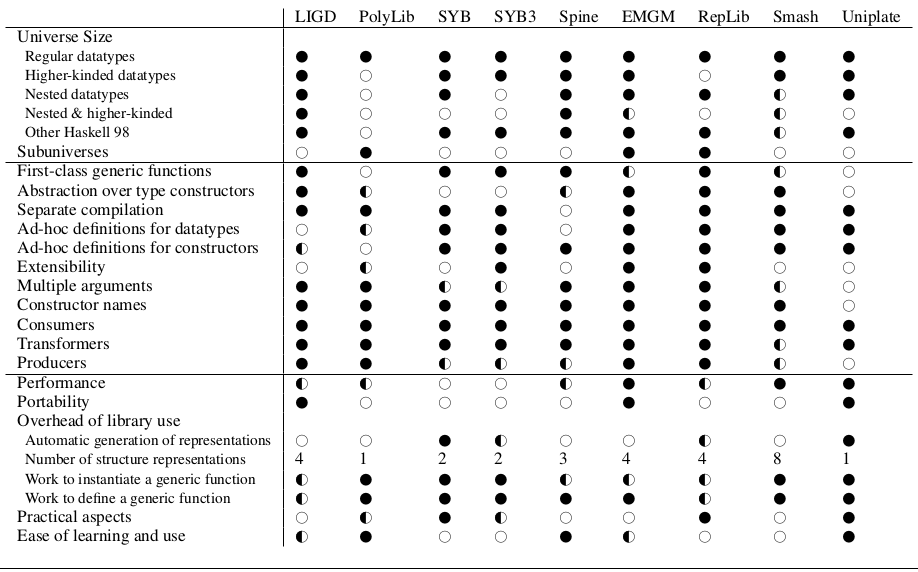
\includegraphics[scale=0.45]{Comparisons.png}
\end{figure}

The starting point for this project is to examine how well the current approach for datatype-generic programming in Scala, and its implementation in the library Shapeless, scores on the criteria defined by \cite{rodriguez2008comparing}. In order to do so, we will closely follow the methodology presented by the authors, and port the collection of programs they use for benchmarking to Scala.

Even in Haskell, for which a great amount of research in the area of generic programming has been done, there is no clear agreement on how a library has to be designed in order to fulfill all the proposed criteria. Different approaches embrace different trade-offs. We do not expect that the only existing approach in Scala will fit all criteria perfectly. Ideally, we would find out exactly which criteria Shapeless lacks, and choose a library to implement based on these results. However, the limited time set for this project forces us to work on benchmarking Shapeless and implementing a new library in parallel. Since the creators of Shapeless state that it was based on SYB, we compared SYB's scores in Figure 1 to the other libraries. Here, we see that EMGM mostly fulfills the criteria that SYB lacks, in addition to scoring quite well in general. These results underlay our decision to choose EMGM as the basis for our library.

\subsection{The Shapeless library}

The current approach to generic programming in the Scala language is presented as the Shapeless library. However, it is important to clarify that the library is not really oriented to generic programming in the form that we as functional programmers expect but is more a library for type safe compile time transformation of data in Scala. In this section we are going to give a brief overview of the library and explain how we can use it for generic programming. For a more detailed explanation please see the official guide\footnote{https://github.com/underscoreio/shapeless-guide}.

Generic representation of types in Shapeless is done through a combination of heterogeneous lists, \scala{HList}, and typed sums, \scala{Coproduct}. Heterogeneous list are type tagged lists that aim to represent case classes through the typed list of their arguments. Furthermore, because a type (\scala{sealed trait} in the case of Scala) may have more than one constructor, the choice between constructors is represented by the \scala{Coproduct}. Shapeless provides the \scala{trait Generic} that we can use to summon the generic representations for our datatypes. 

\begin{lstlisting}[style=scala]
trait Generic[A] {
	type Repr
	def to(value: A): Repr
	def from(value: Repr): A
}
\end{lstlisting}

The \scala{trait} represents an isomorphism between the type we want to have the generic representation \scala{A} and its generic representation \scala{Repr} that is keept abstrat in the trait. We can then use the \scala{trait} to summon, for instance, a generic representation of binary trees:

\begin{lstlisting}[style=scala]
sealed trait BinTree[T]
case class Leaf[T](leaf : T) extends BinTree[T]
case class Bin[T](left : BinTree[T], right : BinTree[T]) extends BinTree[T]

scala> Generic[Bin[Int]]
res1: shapeless.Generic[Bin[Int]]{type Repr = shapeless.::[BinTree[Int],shapeless.::
				[BinTree[Int],shapeless.HNil]]} = anon$macro$3$1@7ead7368
\end{lstlisting}

The actual instance of the \scala{Generic} is generated by the Shapeless library using macros. The pattern to define a generic function is to define a new \scala{trait} and make instances of it for both \scala{HList} and \scala{Coproducts}. In the following code snippet we can see an example of a equality function working on some type \scala{A}.

\begin{lstlisting}[style=scala]
/* Trait representing the Eq typeclass */
trait Eq[A] {
  def eq(x : A, y : A) : Boolean
}

/* Companion object of Eq */
object Eq {
  implicit object IntEq extends Eq[Int] {
    def eq(x : Int, y : Int) = x == y
  }

  /* Instances for HList */
  implicit val hnilEq: Eq[HNil] =
    instance((_,_) => true)

  implicit def hlistEq[H, T <: HList](
    implicit
      hEq : Lazy[Eq[H]],
      tEq : Eq[T]): Eq[H ::: T] =
        instance((xs,ys) => (xs,ys) match {
          case (h ::: t, h1 ::: t1)  => hEq.value.eq(h,h1) && tEq.eq(t,t1)
        })

  /* Instances for Coproduct */
  implicit val cnilEq : Eq[CNil] =
    instance((_,_) => true)

  implicit def coproductEq[H, T <: Coproduct](
    implicit
      hEq : Lazy[Eq[H]],
      tEq : Eq[T]
  ) : Eq[H :+: T] =
    instance((xs,ys) => (xs,ys) match {
      case (Inl(h) , Inl(h1)) => hEq.value.eq(h,h1)
      case (Inr(t) , Inr(t1)) => tEq.eq(t,t1)
      case (Inr(_),Inl(_)) => false
      case (Inl(_),Inr(_)) => false
    })

  implicit def genericEq[A, R](
    implicit
      gen: Generic.Aux[A, R],
      env: Lazy[Eq[R]]
  ) : Eq[A] = instance((x,y) => env.value.eq(gen.to(x),gen.to(y)))

  def geq[A](x : A, y : A)(implicit e : Eq[A]) = e.eq(x,y)
}
\end{lstlisting}

The interface for the generic function \scala{eq} is the last function provided, \scala{geq}. The instance for \scala{Eq[A]} should be automatically derived by the Scala compiler if there exists a generic representation for the type we want to use it on.

\subsection{Experience using Shapeless}

The original author of the library claims that his inspiration for the library was the paper by L{\"a}mmel and Peyton Jones\cite{lammel2005scrap}, thus we thought that a good point to start was to stress out how its approach to generic programming can be compared with others by using the criteria given by Rodriguez et al\cite{rodriguez2008comparing}. However, it turned out that Shapeless focus is on exploiting Scala type system for type safe transformation of code other than the classical functional programming approach to generic programming. For this reason, we found out that we really couldn't evaluate the library with the points given, but we therefore decided that it was more worth it to try out the library with different examples to see how it behaves and until what extent can be used for our purposes.

Using Shapeless for basic types that do not involve higher-kinded types or nested types is straightforward even without type annotations. The library is able to provide a \scala{Generic} instance and actually use it for the generic functions we define. However, for more exotic types this is not straightforward and a lot of type information has to be provided in order to make it work. Also in some cases the compiler is not even able to provide the instance of our generic function even being able to derive the \scala{Generic} instance for the type.

The library has some documentation on the usage with working examples. We feel that the examples given there work, but trying out something different either does not work or requires a lot of extra debugging and tweaking of the implicit resolution system.

\subsection{EMGM in Scala}

This section gives an brief overview of the workings of the EMGM library and how we aim to approach porting it to Scala\footnote{The code for the library along with the test can be found under the folder https://github.com/maffh92/Concepts-of-program-design/tree/master/Development/Generic}. We started this journey by implementing the examples given in the paper introducing EMGM\cite{emgm}.

The main idea behind EMGM is that almost any datatype can be expressed as a combination of standard types. Functions can be defined on these standard types, and users can then use these functions on their own datatypes provided they supply an isomorphism between their types and the standard types. 

The standard types defined by EMGM are \texttt{Unit, Sum} and \texttt{Product}. In Scala, we represent these types as case classes:

\begin{lstlisting}[style=Scala]
case object Unit

case class Product[A, B](a: A, b: B)

sealed trait Plus[A, B]
case class Inl[A, B](a: A) extends Plus[A, B]
case class Inr[A, B](b: B) extends Plus[A, B]
\end{lstlisting}

As an example of how these types are used, consider the snippet showing a normal and then a sum-of-products type for binary trees below:

\begin{lstlisting}[style=Scala]
// Original Binary tree datatype
sealed trait BinTree[T]
case class Leaf[T](leaf: T) extends BinTree[T]
case class Bin[T](left : BinTree[T],right : BinTree[T]) extends BinTree[T]

// Generic representation of Binary tree
type BinTreeRep[T] = Plus[T,Product[BinTree[T], BinTree[T]]
\end{lstlisting}

Rather than defined functions on representation types directly, EMGM defines a \texttt{Generic} typeclass, which encompasses a set of functions on the aforementioned standard types. The rationale behind using a typeclass instead of working directly on type instantiations has to do with extensibility. If, for instance, we were to extend the generic base types with generic lists, we would have to change every function working on the standard types to work on the list type as well. Using typeclasses here allows us to define an instance of it only once. We represented the \texttt{Generic} typeclass as a \scala{trait} in Scala:

\begin{lstlisting}[style=Scala]
  trait Generic[G[_]] {
    def unit: G[Unit]
    def plus[A, B](a: G[A], b: G[B]): G[Plus[A, B]]
    def product[A, B](a: G[A], b: G[B]): G[Product[A, B]]
    def constr[A](n: Name, ar: Arity, a: G[A]): G[A] = a
    def char: G[Char]
    def int: G[Int]
    def view[A, B](iso: Iso[B, A], a: () => G[A]): G[B]
  }
 \end{lstlisting}

In addition to the trait above, there is also a \texttt{Generic2}  trait. The difference between these two is that the \texttt{Generic} class is used to create functions with one single generic argument, where \texttt{Generic2} is used for functions with two generic arguments. Most methods of the \texttt{Generic(2)} types corresponds with a standard type, except one: the view method.  This method first transforms the regular representation to the general representation, such that the other methods of the class can be applied to it. Finally, it translates the result back to its original data type. To do so, it requires a way to do these translations. EMGM solves this by using adatatype representing the existence of an isomorphism between the generic and the regular representation of a type. In Scala, this datatype is represented by the following trait:

\begin{lstlisting}[style=scala]
 trait Iso[A, B] {
    def from: A => B
    def to:   B => A
  }
\end{lstlisting}

As explained in\cite{emgm}, in order to prevent having to explicitly pass the representation types to every generic function call, we use \emph{representation dispatchers}. In Scala, we make implicit instances of these representation dispatchers, allowing the compiler to automatically find the correct instance for all generic types. There are various dispatchers, each aimed at different types. The easiest to implement were the \texttt{Frep} and \texttt{Frep2}, which are used for functor types. The `2' suffix indicates that this type is used for \texttt{Generic2}. \texttt{Frep} is defined as follows:

\begin{lstlisting}[style=scala]
 trait FRep[G[_],F[_]]{
    def frep[A](g1 : G[A]) : G[F[A]]
  }
  \end{lstlisting}

The representation dispatcher for generic types looks as follows:
 
 \begin{lstlisting}[style=scala]
  trait GRep[G[_], A] {
    def grep: G[A]
  }
   \end{lstlisting}
   
For both dispatchers, the \texttt{G[\_]} is expected to be an instance of \texttt{Generic}. EMGM solves this using class constraints. In Scala, we solve this problem by supplying an implicit element. For instance:

\begin{lstlisting}[style=scala]
  class GUnit[G[_]](implicit gg: Generic[G]) extends GRep[G, Unit] {
    def grep: G[Unit] = gg.unit
  }
\end{lstlisting}

The next part was to implement some of  the default functions from the EMGM library\footnote{The library can be found on Hackage: https://hackage.haskell.org/package/emgm-0.4}. We chose functions based on their relevance. For instance, EMGM's \texttt{Show} type seemed superfluous because Scala automatically supplies a overridable \texttt{toString} method, which behaves similarly. The following functions were implemented:
\begin{description}
	\item[Crush] is a generalization of folding.
    \item[Map] is a generic map function, which can be used to map from one type to another
    \item[Collect] collects all values of a given type that occur within a composed type. The result is gathered in a supplied functor, which must be an instance of \texttt{Alternative}
    \item[Everywhere] takes a function from $A \rightarrow A$ for some type $A$, and applies this function whenever it encounters something of this type within a composed structure.
\end{description}

Due the fact that this project is still in an experimental state, not all functions were fully tested. For \texttt{Map} and \texttt{Crush} we supply some tests, but in order to use \texttt{Everywhere} and \texttt{Collect}, a representation dispatcher still has to be implemented. 

As mentioned in section 3, the authors of\cite{rodriguez2008comparing} defined a methodology for testing generic libraries. We have added most of these tests to the library. This includes binary trees, general weighted trees, a composed type representing companies and perfect trees. We have not tried to add a representation for nested general rose trees, as the paper's authors mentioned problems implementing these in EMGM. Unfortunately, we did not succeed in fully implementing any of the functions defined in the aforementioned paper. We therefore only tried to test the data type with the functions listed above. They work for both binary trees and perfect trees.

\section{Results}

Our implementation of the ideas given by EMGM in Scala has very strong limitations compared to its counterpart implemented in Haskell, which can be found on Hackage\footnote{https://hackage.haskell.org/package/emgm-0.4}. These limitations, which are mainly due to problems with higher-kinded types, type-level lambdas and implicit resolution severely  lessen the usability of our library.

The limitations come in two flavours. On one side, for the user, who wants to use the generic functions provided by the library on their own datatype and on the other side, for the user who wants to to implement new generic functions on top of the ones provided by the library. % that is automatically supported by the library without any overhead.

The following two sections will explicate these limitations.

\subsection{Defining new datatypes}

In order to illustrate the first of the limitations, let us suppose that we want, as a user, to use the library on our datatype for representing arithmetic expressions.

\begin{lstlisting}[style=scala, frame=none]
sealed trait Expr
case class Add(x : Expr, y : Expr) extends Expr
case class Val(x : Int) extends Expr
\end{lstlisting}

We will have to define a generic representation and an isomorphism between our datatype and this representation, and the actual implicit definitions that will allow us to use generic functions on it.

\begin{lstlisting}[style=scala, frame=none]
type ExprRep = Plus[Int,Product[Expr,Expr]]

def ExprIso  = new Iso[Expr,ExprRep] {
  def ExprIso = new Iso[Expr,ExprRep] {
    def from: (Expr) => ExprRep = e => e match {
      case Add(x,y) => Inr(Product(x,y))
      case Val(x)   => Inl(x)
    }
    def to: (ExprRep) => Expr = e => e match {
      case Inr(Product(x,y)) => Add(x,y)
      case Inl(x) => Val(x)
    }
  }
} 

implicit def rExpr[G[_]](implicit gg: Generic[G]): G[Expr] = {
  gg.view(ExprIso, () => gg.plus(gg.int,gg.product(rExpr,rExpr)))
}

implicit def GExpr[A,B,G[_]](implicit gg: Generic[G]): GRep[G,Expr] =
  new GRep[G,Expr] {
    def grep : G[Expr] = rExpr(gg)
}
\end{lstlisting}

The problem now arises if we try to use a generic function such as \texttt{everywhere} to 
increment the values in a expression by one:

\begin{lstlisting}[style=scala, frame=none]
val f = (x : Int) => x + 1
val e1 = Add(Val(1), Val(2))
assert(everywhere(f,e1)==Add(Val(2), Val(3)))
\end{lstlisting}

The code above will trigger a compile time error where the compiler tells us that is not able 
to find an instance for \lstinline[basicstyle=\ttfamily\color{white},style=scala]|GRep[Everywhere[Int,_],Expr]|. If we change the code to expose the required type and explicitly bring into scope the implicits that the compiler was not able to find\footnote{This is done by writing the function  \lstinline[basicstyle=\ttfamily\color{white},style=scala]|implicitly[E](implicit e: E) = e| defined in Scala standard library.}, then the code compiles and works as expected. This can be done adding the following two lines:

\begin{lstlisting}[style=scala, frame=none]
type C[X] = Everywhere[Int,X]
implicit val g = implicitly[GRep[C,Expr]]
\end{lstlisting}

A workaround is to add more implicit definitions to our datatype where we do not commit to a specific generic function but just to the shape of the type of the 
generic function.

For example, in order to solve the problem we had before, we could implement several other implicit definitions where the generic type is refined with a type-level lambda that has the "shape" of the type of the generic function we are interested in using.
In our case, the partially applied type of \lstinline[basicstyle=\ttfamily\color{white},style=scala]|Everywhere| is \lstinline[basicstyle=\ttfamily\color{white},style=scala]|({type C[X] = Everywhere[A,X]})#C| where \lstinline[basicstyle=\ttfamily\color{white},style=scala]|A| is a type variable in the context. We can furthermore abstract over the concrete Everywhere , and suppose it works for any generic function with similar signature such as \lstinline[basicstyle=\ttfamily\color{white},style=scala]|({type C[X] = F[A,X]})#C|.
Now we introduce the required definitions:

\begin{lstlisting}[style=scala, frame=none]
implicit def rExprC[D,G[_,_]](implicit gg: Generic[({type C[X] = G[D,X]})#C]): ({type C[X] = G[D,X]})#C[Expr] = {
  gg.view(ExprIso, () => gg.plus(gg.int,gg.product(rExprC,rExprC)))
}
implicit def GExprC[D,G[_,_]](implicit gg: Generic[({type C[X] = G[D,X]})#C]): GRep[({type C[X] = G[D,X]})#C,Expr] =
  new GRep[({type C[X] = G[D,X]})#C,Expr] {
    def grep : ({type C[X] = G[D,X]})#C[Expr] = rExprC(gg)
  }
\end{lstlisting}

And the example we had at the beginning will indeed compile.
Of course, as one can see, this workaround is neither desirable nor scalable as for each generic function we would like to use in our datatype, we would have to define an implicit where the \lstinline[basicstyle=\ttfamily\color{white},style=scala]|GRep| commits to the shape of the function type. This restriction we believe is because the Scala compiler is not as powerfull as Haskell compilers performing type inference under the presence of higher-kinded types and type-level lambdas as we showed before.

\subsection{Adding new generic functions}

Let us now suppose that, as a user, we want to add a new generic function that given, a datatype, will
calculate its size. In order to implement such a function we would start by defining a trait and give and instance of the \lstinline[basicstyle=\ttfamily\color{white},style=scala]|Generic| class for it in
its companion object. Furthermore, we include a method \lstinline[basicstyle=\ttfamily\color{white},style=scala]|size| for easy use.
\begin{lstlisting}[style=scala, frame=none]
trait Size[A] {
  def size_(x : A) : Int
}
object Size {
  implicit object SizeG extends Generic[Size] {..}
  def size[A](a: A)(implicit grep: GRep[Size, A]): Int = {
    grep.grep.size_(a)
  }
}
\end{lstlisting}

Now if we want to use this function we have to explicitly give a type signature, as in the following code snippet:

\begin{lstlisting}[style=scala, frame=none]
"size" should "return the correct size" in {
  val e1 = Add(Val(1), Val(2))
  assert(size[Expr](e1) == 2)
}
\end{lstlisting}
In the example above, the actual implementation is not that cumbersome, but when we try to define more
exotic functions which do not directly comform to the kind (* -> *) we run into trouble as we have to use type-level lambdas to accomplish the generic instances and still Scala won't be able to actually resolve the implicits needed.

For example, in the case of the \lstinline[basicstyle=\ttfamily\color{white},style=scala]|Collect| function we had to "hack" the original \lstinline[basicstyle=\ttfamily\color{white},style=scala]|GRep| companion object to include implicit definitions for the shape of the type of \scala{Collect} to be able to work with the function without further problem.

If we were a regular user extending the library with our custom generic function we wouldn't be able to change the companion object of \scala{GRep} which indeed wouldn't allow us to use the function without any overhead or implicit trickery in our code.

Besides all the limitations we have just mentioned, with the workarounds we discovered we were able to use our library on several datatypes, such as binary trees, perfect trees and more. However, it is clear that a realistic library for generic programming in Scala in the style of EMGM is not very straightforward.

\section{Reflection}

The experience of developing our own library for generic programming in Scala following EMGM's approach has taught us several things. First, we think that maybe it was not the best of ideas to do a project on a topic as complicated as generic programming in Scala with neither previous knowledge of the language, nor more than a very basic idea of generic programming.

The project indeed turned out to be more difficult than expected at first, because at the time we didn't know or even thought about the poor support that Scala offers for the basic building blocks of generic programming such as higher-kinded types or partially applied types. Therefore, we had to spend the greater part of the project not really on porting EMGM to Scala but on hacking workarounds into Scala.

However, through this process we were able to clearly identify the weak points of Scala that make the approach for EMGM fail in the language. Furthermore, we found some workarounds or "hacks" to actually make it work. One of the main difficulties of the project was to understand how Scala's implicit resolution mechanism works in comparison to Haskell's typeclasses, and how to make it work for us.

Besides this, we think that the time we had for the project was really limited compared to the project's size, and combined with our little experience in Scala this resulted in a library that works for the prepared examples but is not really usable otherwise. For a future project it would be interesting to explore how to use specific Scala type system features that cannot be found in Haskell, such as abstract type members, to achieve a better final result.

\bibliographystyle{alpha}
\bibliography{Bibliography}

\end{document}